% !TEX root = WWW.tex
\begin{figure}[!ht]
\centering
\hspace*{-1em}
\subfloat[\small s300$^{\alpha=2.2}$]{
    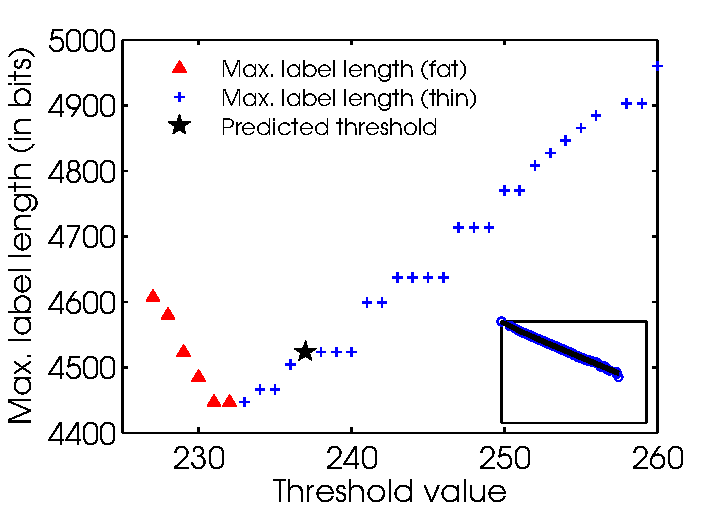
\includegraphics[width=0.55\columnwidth]{Figures/synthetic-data-300K-alpha22-revised.pdf}
}\hspace*{-1.9em}
\subfloat[\small s1M$^{\alpha=2.6}$]{
    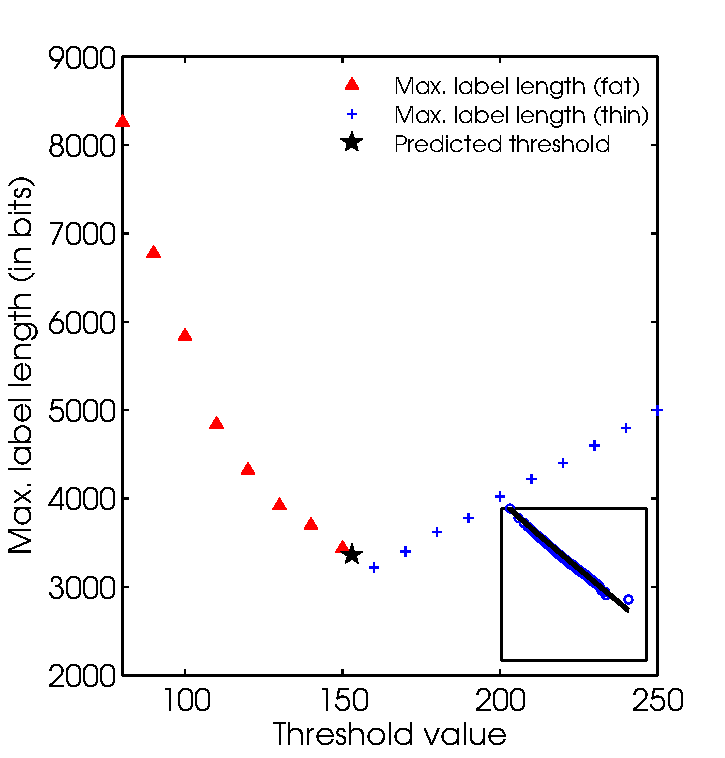
\includegraphics[width=0.55\columnwidth]{Figures/synthetic-data-1M-alpha26-revised.pdf}
}%
\caption{Exemplary maximum label sizes of different threshold values for the synthetic data sets s300$^{\alpha=2.2}$ and s1M$^{\alpha=2.6}$. 
The triangles and crosses represent that for the tested threshold the largest label belong to fat, resp. thin node. The star indicate the position of the predicted threshold.
See~\cite{} for the remaining  figures for synthetic datasets.}%
\label{f:bla}%
\end{figure}